\documentclass{article}
\usepackage{amsmath}
\usepackage{tikz}

\begin{document}

\title{Simple Proof of the Pythagorean Theorem}
\author{}
\date{}
\maketitle

\section*{Theorem Statement}
The Pythagorean Theorem states that, given a right triangle with a hypotenuse of length \(c\) and legs of lengths \(a\) and \(b\), the square of the length of the hypotenuse is equal to the sum of the squares of the lengths of the other two sides:
\[
c^2 = a^2 + b^2
\]

\section*{Algebraic Proof}

Consider a right triangle with side lengths \(a\), \(b\), and hypotenuse \(c\). Construct a large square with side length \(a + b\).
The remaining area in the middle forms a smaller inner square with side length \(c\).

\begin{center}
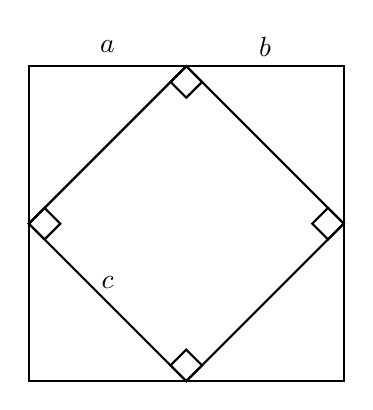
\begin{tikzpicture}

% Outer large square
\draw[thick] (0, 0) -- (4, 0) -- (4, 4) -- (0, 4) -- cycle;

% Inner smaller square
\draw[thick] (2, 0) -- (4, 2) -- (2, 4) -- (0, 2) -- cycle;

% Inner square right angle markers
\draw[thick] (2.0, 0.0) -- (1.8, 0.2) -- (2.0, 0.4) -- (2.2, 0.2) -- cycle;
\draw[thick] (4.0, 2.0) -- (3.8, 2.2) -- (3.6, 2.0) -- (3.8, 1.8) -- cycle;
\draw[thick] (2.0, 4.0) -- (1.8, 3.8) -- (2.0, 3.6) -- (2.2, 3.8) -- cycle;
\draw[thick] (0.0, 2.0) -- (0.2, 2.2) -- (0.4, 2.0) -- (0.2, 1.8) -- cycle;

% Length labels
\node at (1, 4.25) {\(a\)};
\node at (3, 4.25) {\(b\)};
\node at (1, 1.25) {\(c\)};

\end{tikzpicture}
\end{center}

The area \(A_S\) of the outer square is:
\begin{align}
A_S &= (a + b)^2 \\
A_S &= a^2 + 2ab + b^2
\end{align}

The area \(A_t\) of each of the triangles is:
\begin{align}
A_t &= \frac{1}{2}ab 
\end{align}

The area \(A_i\) of the inner square is:
\begin{align}
A_i &= c^2
\end{align}

\begin{center}
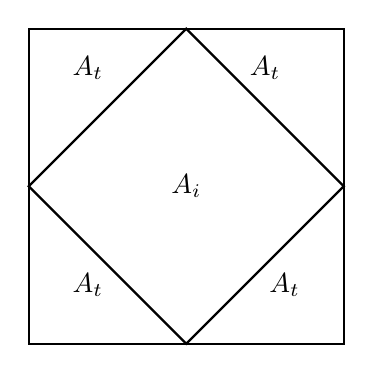
\begin{tikzpicture}

% Outer large square
\draw[thick] (0, 0) -- (4, 0) -- (4, 4) -- (0, 4) -- cycle;

% Inner smaller square
\draw[thick] (2, 0) -- (4, 2) -- (2, 4) -- (0, 2) -- cycle;

% Area labels
\node at (2.0, 2.0) {\(A_i\)};

\node at (0.75, 3.5) {\(A_t\)};
\node at (3, 3.5) {\(A_t\)};
\node at (0.75, 0.75) {\(A_t\)};
\node at (3.25, 0.75) {\(A_t\)};

\end{tikzpicture}
\end{center}

Thus, the area \(A_i\) of the inner square is the difference between the area of the outer square and the sum of the areas of the four inner triangles:
\begin{align}
A_i &= A_S - 4A_t \\
\end{align}

Subtituting the values of \(A_S\) and \(A_t\) calculated above:
\begin{align}
A_i &= a^2 + 2ab + b^2 - 4\cdot\frac{1}{2}ab \\
A_i &= a^2 + 2ab + b^2 - 2ab \\
A_i &= a^2 + b^2 \\
c^2 &= a^2 + b^2 
\end{align}

\end{document}
